%!root = ../main.tex
% 极端气候定义、风险偏好=>风险厌恶程度、家财险定义
\chapter{引言}
\section{研究背景}
% 背景、政策、数据
全球气候变化正在导致极端天气事件的频率和强度显著增加,如图\ref{fig:swissre}所示。随着气候变化及其诱发的自然灾害对我国的影响日益加剧,人民的生活安全和财产保障面临前所未有的挑战。应对气候变化是中国可持续发展的内在要求,也是中国积极参与全球治理、推动构建人类命运共同体的重要体现。党的二十大报告指出,“尊重自然、顺应自然、保护自然,是全面建设社会主义现代化国家的内在要求”,要“提高防灾减灾救灾和重大突发公共事件处置保障能力,加强国家区域应急力量建设”。中国作为一个自然灾害频发的国家,面临的自然灾害类型多样,包括但不限于洪涝、台风、干旱、风雹、低温冷冻和雪灾等。据2023年的统计数据显示,全年各种自然灾害共导致9544.4万人次不同程度受灾,直接经济损失高达3454.5亿元,部分极端天气事件如表\ref{tab:weather}所示。面对逐渐增大的气候变化风险,2023年10月24日,我国政府宣布增发2023年国债,总额达1万亿元,专项用于灾后恢复重建工作和提升国家防灾减灾的整体能力\footnote{资料来源:新华社,\url{https://www.gov.cn/yaowen/liebiao/202310/content_6911405.htm}}。这一战略决策不仅体现了政府对气候变化引发的灾害风险的高度警觉,也彰显了加强防灾减灾工作的紧迫性和重要性。在这一宏观背景下,探讨极端天气是否增大了人们的风险厌恶程度及其具体表现形式,对于了解风险承担者在风险冲击下风险意识的变化,具有重要意义。该研究不仅能够丰富我们对气候变化社会经济影响的理解,还能为制定更为科学、前瞻性的风险管理策略提供理论依据和实践指导。通过深入分析气候变化如何塑造个体和群体的风险认知与决策行为,我们可以更有效地实施风险管理措施,这不仅有助于提高社会的适应能力和韧性,也是推动构建和谐、稳定、可持续发展社会的关键步骤。
\begin{figure}[htbp]
    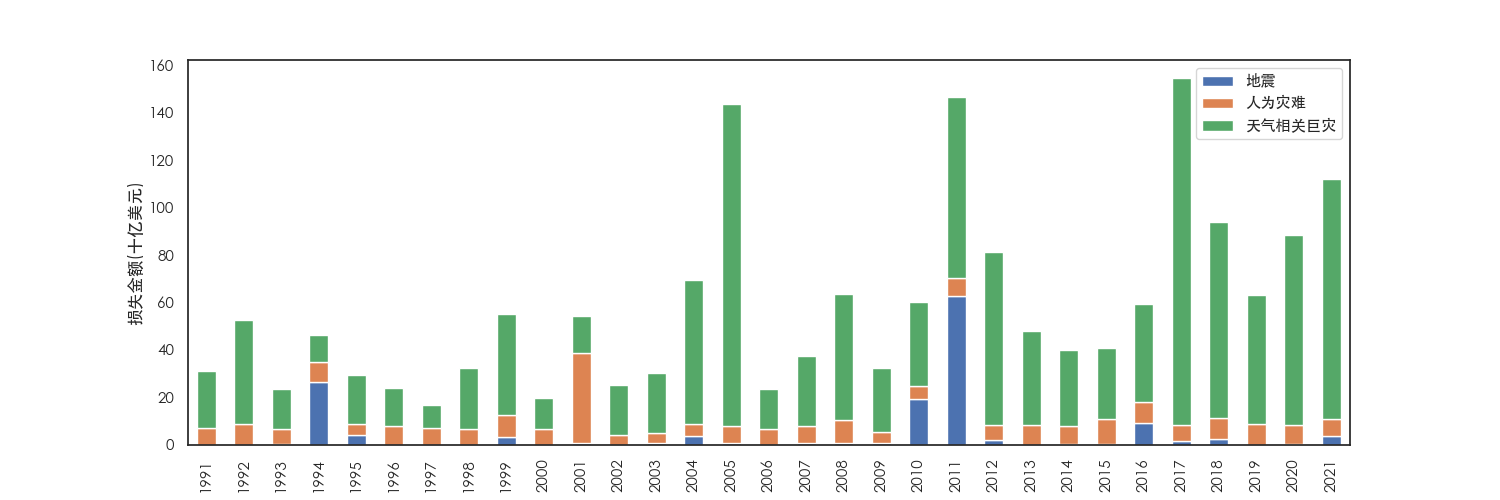
\includegraphics[width=\linewidth]{img/disaster.png}
    \caption{全球自然灾害带来的损失(单位:十亿美元)}\label{fig:swissre}
    资料来源:SwissRe, Sigma, 2024年第1期。
\end{figure}

\begin{longtable}{cccc}
    \caption{2023年我国部分极端天气事件}\label{tab:weather}\\
        \toprule
        \textbf{日期} & \textbf{事件类型} & \textbf{影响地区}&\textbf{直接经济损失金额} \\
        \midrule
        1月13日-16日   & 寒潮        & 福建、江西、云南          &2.79亿元  \\
        3月11日–14日   & 暴雪        & 河南          &3.5亿元  \\
        4月初   & 风雹        & 湖南、贵州、江西          &16亿元  \\
        4月21日-24日   & 低温冷冻和雪灾        & 山西、甘肃等11省          &13.6亿元  \\
        4月下旬   & 洪涝        & 湖南、湖北、福建          &6.2亿元  \\
        5月6日-8日   & 低温冷冻和雪灾        & 云南、新疆等9省          &10.3亿元  \\
        5月初   & 大风、冰雹        & 河北          &13.5亿元  \\
    7月28日-31日   & 超强台风“杜苏芮”        & 福建、浙江、安徽          &147.4亿元  \\
    7月18日–20日   & 风雹        & 内蒙古、山西          &14亿元  \\
        8月初   & 强降雨        & 黑龙江、吉林          &170.9亿元  \\
        8月11日-15日   &台风“卡努”        & 辽宁、黑龙江          &9.2亿元  \\
        10月19日-20日   & 台风“三巴”        & 广东、广西、海南          &58.2亿元  \\
        10月上中旬   & 洪涝        & 湖北、四川、贵州          &4.6亿元  \\
        \bottomrule
    资料来源:应急管理部\footnote{\url{https://www.mem.gov.cn/gk/tjsj/}}
\end{longtable}

随着极端气候事件的频繁发生,人们对自身及财产的安全日益关切。在灾害面前,家庭往往是首当其冲的受害者。但与企业相比,个人和家庭对这些潜在风险的反应可能更为复杂。家庭是否会通过购买家财险来缓解财产损失,以及他们在灾害发生后是否更加倾向于购买保险,对这一问题的观察与分析,有助于加强对灾害冲击-反应的理解。

然而,极端天气下人们对自身及财产安全的关切是否能够持续转化为对保险的需求,尤其是在家庭层面,却是一个相对较少被深入研究的领域。以往研究的对象包括气候变化对企业财产险\citep{杨娜娜2019自然灾害与企业现金持有}或健康险\citep{赵强2021空气污染对商业健康保险需求的影响}需求的影响,以及雾霾天气对健康险需求的影响\citep{2018Something}等,但是对于家庭财产保险的定量研究却相对较少。本研究的选题来源于对这一领域的关注,力图深入了解极端天气极端冲击对家财险需求的影响,填补现有研究的空白。

作为风险管理的手段之一,我国家财险市场的发展始于1980年,是当时中国人民保险公司的基础险种之一。1980年,全国范围内有34200户家庭购买了中国人保的家财险,保险金额为5232万元,保费仅为7万元,仅占国内产险保费总额的0.02\%。到了1989年,全国家财险(包括储蓄性两全险)的投保户数增至76,910,000户,保险金额达1974亿元,保费收入为3.2亿元,占产险保费总额的4.4\%。可以说,我国财产保险的早期发展同时也是家庭财产保险发展的过程\citep{黄英君2008论我国产险公司分散性业务营销模式的创新},塑造了消费者对财产险最早的认知。之后家财险市场发展较为稳定,虽然2022年家财险以67.22\%的增长率成为了保费增速最快的财产险险种,保费达到164亿,但规模占比还不高,2022年末家财险保费收入占财产险保费收入的比例不足1.3\%\footnote{资料来源:中国消费者报,\url{https://www.ccn.com.cn/Content/2023/08-22/1307315925.html}},家财险市场在未来还有很大发展空间。
\begin{figure}[htbp]
    {\centering
    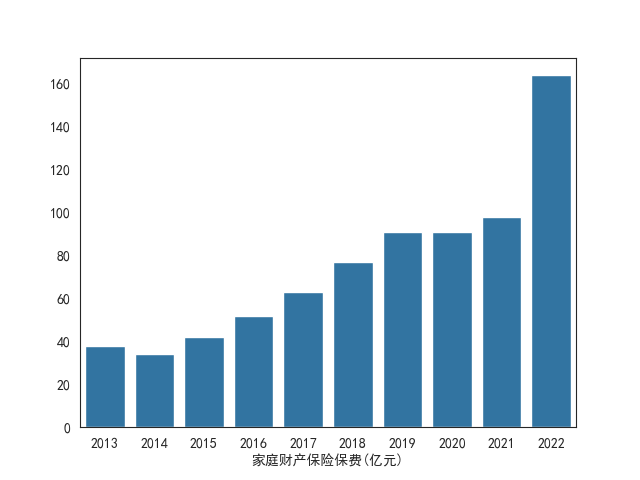
\includegraphics[width=0.8\linewidth]{img/家庭财产保险保费.png}\par }
    \caption{家庭财产保险保费收入}
    资料来源:国家统计总局\protect\footnotemark
\end{figure}

本文将通过深入研究极端天气对家财险需求的影响,探索个人家庭在面对气候变化时的风险管理行为的特征,为政策制定提供更全面的支持。本研究的意义不仅仅停留在学术层面,更涉及到社会和经济发展的多个方面:

首先,从保险行业的角度来看,本研究能够帮助保险公司更好地理解极端天气事件对家财险市场需求的影响。通过分析家庭在面对气候变化时的风险管理行为,保险公司可以更深入了解市场需求,从而优化产品设计、定价策略和营销方案,增强行业的稳定性和可持续发展能力。

其次,从社会科学的角度来看,本研究丰富了人们在面对自然灾害时的行为和决策模式方面的证据。通过分析家庭在极端天气事件前后的保险购买行为,可以揭示人们的风险感知、风险态度和风险应对策略,为心理学、社会学和行为经济学等领域提供丰富的研究素材。这对于理解和预测人们在危机情境下的行为反应,以及设计有效的危机干预和应对措施具有重要意义。

最后,从可持续发展的角度来看,本研究有助于推动社会对气候变化风险的认识和应对。通过揭示保险在气候变化适应和减缓中的作用,可以增强公众的风险意识,提高对保险作为风险管理工具的认识和接受度。这不仅有助于促进保险市场的健康发展,还能够推动形成一种更加理性、科学的社会文化氛围,鼓励个人和社会共同参与到气候变化的应对中来,共同构建一个更加安全、可持续的未来。
\footnotetext{\url{https://data.stats.gov.cn/search.htm?s=}家庭财产保险保费}

\section{研究方法}
极端天气冲击根据ETCCDI\citep{alexander2006global}定义可以分为两大类:极端降水和极端温度。本文选取极端降水作为准自然实验,通过构造双重差分模型,考察发生极端降水后,家财险投保是否有显著提升,以此探究极端天气事件冲击下家庭的行为反应。

本文的结构安排如下:第\ref{chap:2}章是文献综述与研究假说。本章梳理关于气候变化对保险需求影响的研究,探讨风险偏好的相关理论及其影响因素,分析自然灾害如何影响个人和企业的风险偏好,以及这些变化如何反映在保险购买行为上。在文献综述的基础上,提出本研究的三个主要假说。这些假说的提出基于现有文献的不足和本研究的独特视角,旨在填补关于家庭财产保险需求对极端天气事件反应的研究空白。

第\ref{chap:3}章研究设计,将详细介绍本研究所采用的方法论框架、数据来源及处理方式、以及模型设定和变量定义。首先,界定极端天气事件的范围,并根据ETCCDI标准选取极端降水作为研究重点。接着,将描述样本选择的过程,包括数据的时间和空间范围,以及数据清理的具体步骤。最后,详细阐述所采用的计量经济模型,包括基础的回归分析和双重差分(DID)方法,并解释模型中各变量的经济含义及其预期的作用。

第\ref{chap:4}章实证分析,对实证结果进行分析讨论。本章首先展示描述性统计数据,以揭示样本的基本特征。随后,报告回归分析的结果,包括基础回归和DID回归模型的估计结果,以及对模型稳健性的检验。此外,我们还将探讨极端天气事件对保险赔付和续约行为的影响,通过Logit回归分析来深入理解居民和保险公司在灾害后的行为变化。

第\ref{chap:4.1}章主要是扩展问题的实证结果,主要讨论地理位置、保单购买时间、保险标的价值和城乡环境等不同时,极端天气对家庭购买家财险的差异,进一步加强本文基本问题的逻辑性。

第\ref{chap:5}章总结本研究的主要发现,并讨论其对保险业和政策制定的潜在影响。我们将回顾研究假设的验证情况,探讨极端天气事件对家庭风险偏好和保险需求的影响机制,并提出未来研究的可能方向,并就如何提高家庭财产保险市场的适应性和效率提出建议。

\chapter{文献综述与研究假说}\label{chap:2}
\section{文献综述}

本文主要从两个角度梳理国内外相关文献:一是自然灾害对人类行为的影响,二是不同保险需求的影响因素。

\subsection{自然灾害对风险偏好的冲击}

自然灾害会对企业风险偏好产生影响,作用机制之一是获得性启发\citep{tversky1973availability},即人们倾向于依赖最容易回忆起的信息来做出判断,典型的例子是位于台风路径上的企业更偏好持有现金\citep{杨娜娜2019自然灾害与企业现金持有}或调整债务结构\citep{shao2024typhoons}以应对风险。有研究基于获得性启发理论\citep{0Do},指出尽管飓风并未实质性地改变未来飓风发生的概率,管理者仍倾向于通过增加现金储备来应对这种突如其来的风险,但不同距离灾区公司的反映是不同的,灾区公司受到了飓风的直接影响,因此它们的现金持有量出现了显著的下降,现金水平平均下降了约1400万美元。邻近区域公司虽然未直接受到飓风的影响,但由于地理位置接近灾区,飓风事件对它们的管理者来说是显著的,现金持有量平均增加了1.1\%。这种增加是暂时的,随着时间的推移,现金持有量逐渐回到了飓风前的水平。其他地区距离飓风灾区较远,飓风事件对它们的显著性较低。该研究的发现支持了显著性理论的观点,即决策者的注意力容易被显著事件所吸引,从而在风险评估中给予这些事件过高的权重。但随着台风发生次数的增加,管理层的过度反应现象有所减弱,这表明经验的积累可能有助于提高企业对自然灾害的反应效率。

而家庭侧风险偏好影响因素方面,大多数研究主要从个体的角度出发,例如以收入\citep{石双2018收入与风险偏好}、资产总额\citep{卢亚娟殷君瑶2021户主风险态度对家庭金融资产配置的影响研究}、年龄\citep{王晶2021年龄结构}、健康状况\citep{雷晓燕2010中国家庭的资产组合选择}、教育程度\citep{梁立俊2018受教育程度与主客观风险偏好}、职业\citep{赵颖2017中国劳动者的风险偏好与职业选择}、性别\citep{徐小华2019女性劳动参与会影响家庭资产配置风险偏好吗}等为主要研究对象。例如有研究利用CHFS数据,采用Probit、Tobit模型及倾向得分匹配法(PSM),从整体和城乡两个维度出发,深入研究了户主的风险态度对家庭金融资产配置的影响\citep{卢亚娟殷君瑶2021户主风险态度对家庭金融资产配置的影响研究}。研究发现,风险偏好的家庭表现出更高的金融资产参与率和资产占比,且其对金融市场,特别是风险市场的参与行为更为积极。进一步的分析揭示,风险偏好的家庭在风险性金融资产投资上占据主导地位,尤其是在股票方面表现最为显著;相反,家庭越厌恶风险,则其对股票的投资越低。在考察城乡差异时,研究发现户主风险态度对于家庭金融资产选择产生不同影响,尤其是在城镇家庭的风险性金融资产投资方面,风险态度的影响更为显著。

外生事件冲击方面,有研究以中国2003-2005年发生的4次地震为案例,利用国家统计局城镇住户调查数据,通过双重差分法的研究方法,探讨地震对城镇家庭风险偏好的影响及其背后的机制\citep{章元0地震冲击对风险偏好的影响}。地震显著提高了城镇家庭的风险厌恶程度。尤其是距离震中越近的家庭,在地震发生后,购买彩票的概率和支出下降越为显著。这一结果揭示了地震引起的风险预期上升和负向情绪冲击是重要的机制。进一步分析显示,距离震中越近的家庭,其震后非储蓄性保险支出以及用于缓解负向情绪的消费支出上升越多。这意味着地震对家庭风险偏好的影响,不仅体现在经济决策上,还体现在对非储蓄性保险和消费行为的调整上。

风险偏好可以通过商业保险购买决策体现,即风险偏好与商业保险购买之间存在正向关系\citep{宋章良2021我国中老年家庭风险偏好对商业保险购买行为的影响研究},但这一现象的主要原因在于反向因果关系,即高风险偏好的家庭更倾向于购买投资型保险而非保障型保险,与此同时该群体的人均收入较高。也有观点认为购买商业保险也会改变家庭风险偏好\citep{孙武军2023商业健康保险的配置能够改变家庭的风险偏好吗},其以2017年中国家庭金融调查(CHFS)数据为基础,将家庭风险偏好划分为主观和客观两个方面,旨在深入探讨商业健康保险配置对我国居民家庭主客观风险偏好的实证影响。通过采用有序Probit模型进行估计,研究在控制了多个关键因素(包括人口统计特征、健康状况、家庭经济状况以及社会保险持有情况)的基础上,如何处理可能存在的内生性问题。研究的主要发现表明,家庭配置商业健康保险能够显著提高家庭的主客观风险偏好。此外,通过对异质性分析的深入研究,发现这种正面影响在低收入家庭中尤为显著,而在高收入家庭中则作用较为微弱。

总体而言,自然灾害对风险偏好影响的研究在企业侧研究更为充分,而对家庭侧风险偏好的研究主要集中在地震、台风等巨灾风险如何影响家庭金融资产配置、消费行为等方面,对极端天气事件如何塑造家庭风险偏好的研究相对较少。本文将探究极端天气冲击对家庭风险偏好的影响,以探究气候变化如何塑造人类行为。

\subsection{极端天气冲击对不同种类保险需求的影响}

一般认为极端天气是指气象要素的极端值,包括极端温度、极端降水、极端风速、极端湿度、极端干旱等\citep{傅良2022ECMWF,吴大明2021近年来全球极端天气气候事件情况及影响分析}。极端天气事件是指在一定时间和空间范围内,气象要素的极端值或极端变化,如暴雨、洪水、干旱、飓风、暴风雪等。得益于广泛的数据积累,有研究表明极端气温和降水近几十年来的强度和频率发生了变化\citep{ummenhofer2017extreme}。极端天气事件的发生频率和强度都在不断增加,给人们的生活和财产带来了巨大的风险和损失。极端天气事件对保险需求的影响是一个备受关注的课题,国内外学者已经开展了大量的研究。关于极端天气冲击对保险需求的影响,有关研究主要集中在寿险、健康险和农险上,对家财险的研究较少。

健康险方面,空气污染水平对健康险的购买或退保的决策产生的显著影响\citep{2018Something},每日空气污染水平每增加一个标准差,当天销售的保险合同数量增加了7.2\%。而在考虑购买后的条件下,即在冷静期内,相对于订单日期水平,每日空气污染水平每减少一个标准差,退保概率增加了4.0\%,研究还探讨了多种可能的机制,发现了对投射偏差和显著性的最有力支持。也有研究旨在探究空气污染对中国居民商业健康保险需求的影响大小\citep{赵强2021空气污染对商业健康保险需求的影响},利用2011年至2016年秦岭淮河地区84个地级市的宏观数据,采用模糊断点回归设计和中国北方集中供暖政策的准自然实验方法,旨在深入了解空气污染对中国居民商业健康保险需求的影响。结果显示,空气污染对商业健康险需求存在显著的正向影响,特别是PM2.5污染物的排放浓度每提升1\%,商业健康保险密度提高1.098\%。即便在考虑六种不同污染物指标的情况下,估计结果仍然趋近一致。值得关注的是,从2013年开始,我国经历了大范围持续的雾霾天气,伴随着新闻媒体报道频率的增加。这导致居民对空气污染的敏感度和重视度逐渐提高,进而反映在对商业健康保险的购买上。

而对于极端天气冲击对健康险需求的影响机制,研究观点主要集中在极端天气冲击影响的个人风险偏好。例如有研究认为空气污染提升了个人的风险感知,进而引起健康保险需求增加\citep{宋平凡2022空气污染}。其基于2006—2016年中国283个地级以上城市的数据,系统考察了空气污染对健康保险需求的实证影响,采用百度指数作为风险感知的代理变量,并运用中介效应模型验证了空气污染对健康保险需求的影响机制。结果显示,通过百度指数体现的风险感知效应是空气污染引起健康保险需求增加的重要途径,并且工具变量中介效应模型的实证结果进一步支持了这一结论。还有研究认为气候变化增加了居民对气候风险和健康的关注\cite{zhong2022exposure},其利用CHARLS的数据集研究了异常高温对居民购买商业健康保险的影响,发现,随着异常温度每升高1°F,人们购买商业健康保险的概率增加了6\%。此外,性别和地域因素也显得尤为重要,研究表明异常高温对女性、南方居民和东部居民的商业健康保险需求产生更为显著的影响。其认为异常高温对商业健康保险需求的影响机制包括:增加了居民对气候风险的关注,使其更倾向于购买健康保险以规避潜在的健康风险;异常高温对健康的实质性影响也使居民更加关注自身的医疗保障需求。

极端天气冲击对寿险需求也有一定的的影响。例如对于欧盟成员国,有研究采用面板模型,研究保费金额和温室气体排放的关系\citep{melnychenko2021influence},根据其实证研究的结果,每千吨温室气体排放的增加导致寿险保费金额增加17万欧元,具有显著性。而影响机制方面,有观点研究2013年德国洪水对个人的冲击\citep{avdeenko2021impact},认为这种变化是风险厌恶选择导致高风险地区人寿保险需求的增加,通过幸福感的变化来介导,从而解释了风险偏好的改变。

财险方面,天气灾害对汽车出险有一定的影响,有关研究发现近年来天气灾害致汽车出险的数量明显增加\citep{张翠华2020天气灾害致车险理赔的风险分析},其研究数据集为河北省2004-2018年天气灾害致车险理赔事故,研究发现主导汽车出险的天气灾害主要包括暴雨、涉水、冰雹和暴风,在不同地区出险数量存在明显的差异。

其他财险险种方面的研究主要集中在农业保险领域,例如研究极端天气冲击对农险需求的影响\citep{胡新艳2021气候变化},通过地级市气候数据和农户微观数据进行匹配,进行了实证分析。研究发现,气候变化在显著促进农户农业保险购买行为方面发挥了关键作用,但在不同生产目的的农户中存在异质性影响。具体而言,当农户的经营目标从满足自家消费转向为追求市场利润时,其购买农业保险的需求更为强烈。进一步分析表明,气候变化导致的两类农业风险对农户购买农业保险的中介作用存在差异。土壤退化风险由于具有渐进性,农户能够在农业生产之前通过调整生产要素供给来降低风险损失,因此对农业保险的需求较为低迷。相反,病虫害风险属于突发性风险,农户难以通过事前风险防控来分散风险,从而强化了其对农业保险的需求。

此外还有研究极端天气冲击对信贷保证保险需求的影响的研究\citep{张钦2017高寒生态脆弱区农户对气候变化的适应需求},以甘南高原为研究区域,通过对500份农户调查问卷的分析,揭示了气候变化对不同区域和生计方式的农户产生的影响及其适应需求。研究发现,农户在适应极端天气冲击的过程中,对基础设施的需求最为迫切,紧随其后的是对信息和生产技术的需求。进一步分析表明,不同区域和生计方式的农户对适应极端天气冲击的需求存在显著差异。在区域方面,纯牧区和农区农户对基础设施的需求最为强烈,而半农半牧区农户更加关注信息的获取。而在生计方式上,纯农户对信贷保险的需求最为迫切,而一兼户和二兼户则更加倚重基础设施的提升。进一步的分析揭示了影响不同适应需求的关键因素,如自然资本和物质资本对生产技术需求的影响,自然资本和人力资本对信息需求的影响,人力资本和金融资本对基础设施需求的影响,以及多个因素共同影响信贷保险需求。

总体而言,国内外关于极端天气冲击对保险需求的影响研究主要集中在健康险、寿险和农险领域,而对于家庭财产保险的研究相对较少。本文将从家庭财产保险的角度出发,深入探究极端天气冲击对家庭财产保险需求的影响机制,填补现有研究的空白。

\section{研究贡献与研究假设}
本文的研究贡献主要体现在以下几个方面:

第一,本文填补了国内关于极端天气事件对家庭财产保险需求冲击的研究空白,为我国家庭财产保险需求的研究提供了新的视角。已有的极端天气研究大多以企业 \citep{0Do}或是健康险\citep{赵强2021空气污染对商业健康保险需求的影响}、农险\citep{胡新艳2021气候变化}为主,覆盖的灾害范围往往是地震、台风等一次性巨灾冲击,对家庭和持续气候变化的关注则较少。

第二,本文通过海量数据的实证分析,深入探究了极端天气事件对家庭财产保险需求的影响机制,探究了灾区和非灾区家庭财产保险需求的差异,为政府和监管机构制定相关政策提供了参考。

最后,本文通过实证研究,为社会科学领域研究气候变化对于人类行为和决策的深刻洞察提供了新的案例,为其他学科的研究提供了新的视角。

本研究旨在探讨极端天气事件如何影响家财险需求,进而研究人们的风险偏好在极端天气事件影响下的变化。本文将从时间维度和空间维度两个角度出发,提出以下三个研究假设:

首先,在时间维度上,极端天气事件的发生会直接影响居民的风险感知,使其对极端天气事件的风险有了更为直观的认识,居民的风险偏好可能会发生变化,从而影响其对家财险的需求。类似于台风路径下的企业持有现金\citep{0Do}和雾霾增加健康险购买\citep{赵强2021空气污染对商业健康保险需求的影响},根据获得性启发理论\citep{tversky1973availability},人们倾向于依赖最容易回忆起的信息来做出判断。极端天气事件因其罕见和强烈的影响,往往会在居民心中留下深刻印象。这种直观的记忆使得居民在评估风险时更可能高估极端天气事件的发生概率,从而影响他们的风险感知。并且当人们在面对持续的风险时,可能会发展出适应性的行为和心理机制\citep{gigerenzer2011heuristic}。在经历了极端天气事件后,居民可能会调整自己的生活方式和消费习惯,以适应这种风险。这种适应性行为可能包括购买保险,以减少未来可能的经济损失。因此本文认为极端天气事件发生后,居民由于直接感知到面临极端天气事件的威胁,其居民风险感知将显著提高,从而导致他们的风险偏好增加,表现为对家财险需求的增加。基于以上分析,本文提出如下研究假说:

\begin{hyp}[H\ref{hyp:1}] \label{hyp:1}
    发生极端天气事件后,居民风险感知增加,风险偏好显著提升购买家财险的需求增加。
\end{hyp}

其次,在空间维度上,临近灾区的地区虽然未直接受灾,但由于地理位置接近灾区,极端天气事件对其风险偏好的影响可能显著\citep{0Do},导致家财险需求显著增加。临近灾区的地区可能会经历风险传递效应,即直接灾害的影响通过心理、经济和社会网络传递给周边地区。这种效应可能导致居民对潜在灾害的担忧增加,从而提高了他们对保险产品的需求。并且目睹或听闻邻近地区的灾害事件,可能会改变居民的心理预期,使他们更加关注自身的安全和财产保护。这种心理上的变化可能会导致居民采取更为保守的风险管理策略,比如购买家财险等。基于以上分析,本文提出如下研究假说:

\begin{hyp}[H\ref{hyp:3}] \label{hyp:3}
    发生极端天气事件后,临近的地区对风险厌恶增加显著,家财险需求显著增加。
\end{hyp}

最后,在空间维度上,灾区虽然直接受灾,但由于极端天气造成的直接损失可能相对有限,直接受灾或是频繁受灾的地区风险偏好可能并未显著增加\citep{shao2024typhoons},即家财险需求并未显著增加。具体而言,受灾地区的居民可能对极端天气事件有更深刻的认识和更高的风险感知。但一方面,这并不意味着他们的风险偏好会随之增加,居民可能通过其他方式来管理和降低风险,如加强房屋建设标准、改善基础设施等,从而减少了对保险的需求。另一方面,受灾地区的居民可能会发现,即使购买了家财险,也无法完全避免极端天气事件带来的损失,从而对家财险的效用产生怀疑,进而降低了对家财险的需求。基于以上分析,本文提出如下研究假说:

\begin{hyp}[H\ref{hyp:2}] \label{hyp:2}
    发生极端天气事件后,直接受到极端天气事件冲击的地区对风险偏好影响有限,家财险需求并未显著增加。
\end{hyp}
